
% UC... specificare App o Server -> UCA / UCS

%\centering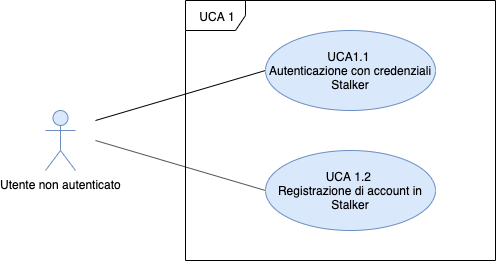
\includegraphics[scale=0.8]{sezioni/UseCase/Immagini/Panoramica.png}
\section{UCS ?}%kite level
\begin{itemize}
    \item \textbf{Nome:} Modifica parametri dell'organizzazione\\
    \item \textbf{Attori primari:} Amministratore gestore\\
    \item \textbf{Precondizione:} L’amministratore dispone di almeno un'organizzazione.\\
    \item \textbf{Postcondizione:} L’amministratore ha modificato i parametri desiderati dell'organizzazione e le modifiche ono state salvate nel sistema.\\
    \item \textbf{Scenario principale:} L'amministratore deve scegliere l'organizzazione che vuole modificare, selezionare la funzionalità di modifica dell'organizzazione e quindi procedere con il cambiamento dei dati.'\\
    \item \textbf{Inclusioni:} UCS Selezione organizzazione
    \item \textbf{Flusso di eventi:}
    \begin{enumerate}
        \item UCS Selezione organizzazione;
        \item L'amministratore ha la possibilità di modificare i campi delle informazioni dell’organizzazione (UCS )
        \item L’amministratore ha la possibilità di modificare il luogo di tracciamento dell’organizzazione [UCS 3.5]
    \end{enumerate}
\end{itemize}